\chapter[short]{线性方程组}

\section{矩阵正交化}
对于矩阵 $A=\{v_1,v_2,\dots,v_n\}$ 找出构成该矩阵列空间极大无关组的过程叫正交化。常用的正交化手段有格拉姆-施密特(Gram-Schmidt)
正交化方法:它在选定主方向向量以后,通过不断减去其余方向在该方向上的投影得到正交基。
给出正交非归一化的传统格拉姆施密特方法:
\begin{center}
    \begin{minipage}{.7\linewidth}
        \begin{algorithm}[H]
            \caption{\text{Non-normalized Gram-Schmidt}}
            \KwIn{$A=\{v_1,v_2,\dots,v_n\}$}
            \KwOut{$Q=\{q_1,q_2,\dots,q_n\}$}
            \For{$j=1\colon n$}
            {
                $v_j=x_j$\;
                \For{$k=1\colon j-1$}
                {
                    $v_j\leftarrow v_j-(\frac{v_k^Tx_j}{v_k^Tv_k})v_k$\;
                }
            }
        \end{algorithm}
    \end{minipage}
\end{center}
注意以上算法给出的是一组\emph{正交非单位}向量组,如果需要获得一组\emph{正交单位}向量组,使用以下的经典施密特算法(Classical Gram-Schmidt):
\begin{center}
    \begin{minipage}{.7\linewidth}
        \begin{algorithm}[H]
            \caption{\text{Classical Gram-Schmidt, CGS}}
            \KwIn{$A=\{v_1,v_2,\dots,v_n\}$}
            \KwOut{$Q=\{q_1,q_2,\dots,q_n\}$}
            \For{$j=1\colon n$}
            {
                $v_j=x_j$\;
                \For{$k=1\colon j-1$}
                {
                    $v_j\leftarrow v_j-(q_k^Tx_j)v_k$\;
                }
                $q_j=v_j/\Vert v_j\Vert_2$\;
            }
        \end{algorithm}
    \end{minipage}
\end{center}

经典的施密特正交化方法缺乏固有的数值稳定性,举如下简单的例子:在计算完成第一列正交基后,假设第二列正交基出现误差,使得$q_1^Tq_2=\delta$,
那么,在后续的 CGS 过程中,该误差并不会减小:
\begin{align*}
    v_3      & =x_3-(q_1^Tx_3)q_1-(q_2^Tx_3)q_2                         \\
    q_2^Tv_3 & =q_2^Tx_3-(q_1^Tx_3)\delta -(q_2^Tx_3)=-(q_1^Tx_3)\delta \\
    q_1^Tv_3 & =q_1^Tx_3-(q_1^Tx_3)-(q_2^Tx_3)\delta=-(q_2^Tx_3)\delta
\end{align*}
由于数值计算是有限精度运算,正交化某列时的误差无可避免的。这使 CGS 过程中误差随着正交列增多而积累,直至错误。更多关于格拉姆
施密特正交化的误差特性,可以参考 Bjorck 的分析 \cite{BJORCK1994297}。为解决该问题,目前更普遍使用修正格拉姆施密特正交化
(Modified Gram-Schmidt)方法:
\begin{center}
    \begin{minipage}{.7\linewidth}
        \begin{algorithm}[H]
            \caption{\text{Modified Gram-Schmidt, MGS}}
            \KwIn{$A=\{v_1,v_2,\dots,v_n\}$}
            \KwOut{$Q=\{q_1,q_2,\dots,q_n\}$}
            \For{$j=1\colon n$}
            {
                $q_j=v_j/\Vert v_j\Vert_2$\;
                \For{$k=j+1\colon n$}
                {
                    $v_k\leftarrow v_k-(q_k^Tv_k)q_j$\;
                }
            }
        \end{algorithm}
    \end{minipage}
\end{center}

修正格拉姆施密特方法的区别在于关键的消去投影向量步骤:
\begin{equation}
    \text{CGS}\colon v_j\leftarrow v_j-(v_k^Tx_j)v_k\qquad \text{MGS}\colon v_k\leftarrow v_k-(v_j^Tv_k)v_j
\end{equation}
从 MGS 出发,考察 CGS 中遇到的问题。依然假设有不正交的向量 $q_1^Tq_2=\delta$,则 $v_3$ 的计算过程如下:
\begin{align*}
    j & =0 \quad v_3=x_3                                 \\
    j & =1 \quad v_3^{(1)}=v_3^{(0)}-(q_1^Tv_3^{(0)})q_1 \\
    j & =2 \quad v_3^{(2)}=v_3^{(1)}-(q_2^Tv_3^{(1)})q_2
\end{align*}
假设 $v_3^{(2)}$ 即为最终结果,观察误差的传播情况,首先考察对 $q_2$ 的正交性:
\begin{equation}
    q_2^Tv_3=q_2^Tv_3^{(1)}-q_2^Tv_3^{(1)}=0
\end{equation}
考察对$q_1$的正交性,由正交过程有:
\begin{equation}
    \begin{aligned}
        q_1^Tv_3       & =q_1^Tv_3^{(1)}-(q_2^Tv_3^{(1)})\delta \\
        q_2^Tv_3^{(1)} & =q_2^Tv_3^{(0)}-(q_1^Tv_3^{(0)})\delta \\
        q_1^Tv_3^{(1)} & =q_1^Tv_3^{(0)}-q_1^Tv_3^{(0)}=0
    \end{aligned}
\end{equation}
可发现其误差项的累计速度是乘方级的,相比于 CGS 的线性要小的多:
\begin{equation}
    q_1^Tv_3=-(q_2^Tv_3^{(0)}-(q_1^Tv_3^{(0)})\delta)\delta=-q_2^Tv_3^{(0)}\delta+q_1^Tv_3^{(0)}\delta^2
\end{equation}
Bjorck\cite{BJORCK1994297} 也给出了 MGS 方法的数值特性分析。

\subsection{程序实现}
按上节给出的 MGS 算法进行实现,ppx 中的函数原型如下:
\begin{tcolorbox}
    \begin{center}
        \begin{minipage}{.92\linewidth}
            \begin{lstlisting}[language=C++]
auto MGS(A:mat)->mat;
\end{lstlisting}
        \end{minipage}
    \end{center}
\end{tcolorbox}

下面给出具体的使用例,如对随机病态矩阵进行正交化,并给出正交化残差。通过希尔伯特矩阵构造病态矩阵 $A=H+0.00001I$
\begin{tcolorbox}
    \begin{center}
        \begin{minipage}{.92\linewidth}
            \begin{lstlisting}[language=C++]
auto A = eye<100>();
A += hlib(A);
auto Q = MGS(A);
std::cout << norm1(Q.T() * Q - eye<100>()) << std::endl;
\end{lstlisting}
        \end{minipage}
    \end{center}
\end{tcolorbox}
得到残差为 2.1554e-11,而使用 CGS 方法得到残差为 2.9912。

\section{QR 分解}

在格拉姆-施密特正交化过程中,每次由公式 $q_j=v_1-\sum_k^{j-1}(q_j^Tv_k)v_k$ 得到列向量,写出该过程变换表达式,发现变换矩阵形成
上三角格式,系数与正交投影系数相关:
\begin{equation}
    \begin{cases}
        q_1 & =c_{11}v_1                                     \\
        q_2 & =c_{12}v_1+c_{22}v_2                           \\
        q_3 & =c_{13}v_1+c_{32}v_2+c_{33}v_3                 \\
            & \vdots                                         \\
        q_n & =c_{1n}v_1+c_{2n}v_2+c_{3n}v_3+\dots c_{nn}v_n
    \end{cases}
\end{equation}
整理成矩阵表达式:
\begin{equation}
    \label{CGS_QR}
    \underbrace{\left(q_1,q_2,\dots,q_n\right)}_Q=\underbrace{\left(v_1,v_2,\dots,v_n\right)}_A
    \underbrace{
        \begin{bmatrix}
            c_{11} & c_{12} & \cdots & c_{1n} \\
                   & c_{22} & \cdots & c_{2n} \\
                   &        & \ddots & \vdots \\
                   &
                   &        & c_{nn}
        \end{bmatrix}
    }_C
\end{equation}
得到 $Q=AC$。定义矩阵 $R=C^{-1}$,则由 \eqref{CGS_QR} 有矩阵分解 $A=QR$,其中 Q 是正交矩阵,而 R 是上三角矩阵。这种矩阵分解
方式称 QR 分解。使用分解矩阵代替原矩阵的好处在于:正交矩阵 Q 的特性使得参与运算的对象精度能良好保持,不会随着数值运算过程一直累计,、
而上三角矩阵作为线性代数最基础的研究对象,可以被多种技巧处理。QR 分解除了通过上节中 MGS 实现,还能通过如豪斯霍尔德(Householder)
变换,吉文斯(Givens)变换等多种方法实现。其分解本身是解超定方程组、矩阵极大无关组,奇异值分解的基础。总的来说,QR 分解是矩阵
正交分解中最重要内容之一。

\subsection{分解原理}
对于矩阵 $A$,QR 分解目标是将其转化为上三角型与正交矩阵的乘积:
\begin{equation}
    \begin{bmatrix}
        \quad & \quad & \quad \\
        \quad & \quad & \quad \\
        \quad & A     & \quad \\
        \quad & \quad & \quad \\
        \quad & \quad & \quad
    \end{bmatrix}_{m\times n}=
    \begin{bmatrix}
        \quad & \quad & \quad \\
        \quad & \quad & \quad \\
        \quad & Q     & \quad \\
        \quad & \quad & \quad \\
        \quad & \quad & \quad
    \end{bmatrix}_{m\times n}
    \begin{bmatrix}
        r_{11} & r_{12} & \cdots & r_{1n} \\
               & r_{22} & \cdots & r_{2n} \\
               &        & \ddots & \vdots \\
               &
               &        & r_{nn}
    \end{bmatrix}_{n\times n}
\end{equation}
回想 MGS 中形成矩阵 R 过程,它等价于对原矩阵 A 每列叠加初等变换矩阵:这些初等变换矩阵首先是正交矩阵,并且作用于另一矩阵后能操作其行列,
这种作用还能相互叠加。这引出了 QR 分解的另一种思路:如果存在某正交矩阵能消去矩阵的特定行列,那么累计这种矩阵作用,最终就能得到 QR 分解
中的上三角矩阵 R,而这种累计作用合成来的矩阵正是 Q 矩阵。豪斯霍尔德变换与吉文斯变换正是这种正交变换,它们能消去矩阵某列指定位置以下的元素,或交换矩阵指定位置的元素。

\subsection{Householder 变换}
豪斯霍尔德(Householder)变换,又称镜射变换,由如下公式定义:
\begin{equation}
    H_ux=(I-2uu^{T})x
\end{equation}
其中的 $H_u$ 是由 $u$(householder 因子)决定的镜射变换矩阵。如图 \ref{householder_transform} 如果把矢量 $x$ 看作光线,
那么 $u$ 就是镜面的方向,$H_ux$ 就是反射的方向。选择待变换矩阵第 $i$ 列向量作为原始向量,选择 $e_i$ 作为反射的目标向量,记录
豪斯霍尔德变换因子 $u_i$。重复该过程于每一列中,最后记录变换矩阵的乘积为 $Q^T$,残余矩阵为上三角矩阵 $R$。
\begin{figure}[htbp]
    \centering\label{householder_transform}
    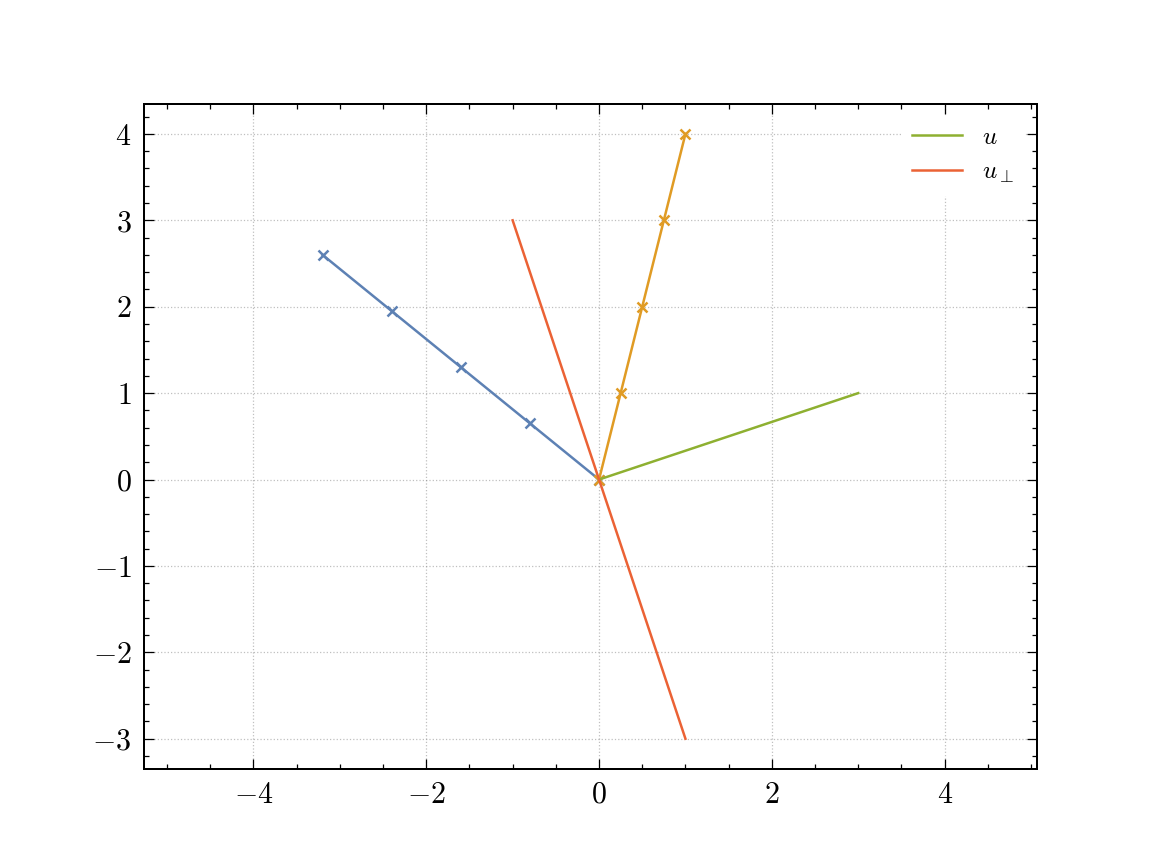
\includegraphics[width=\textwidth]{HouseHolder.png}
    \caption{镜射变换示意图}
\end{figure}
